\documentclass[12pt]{beamer} %
\usepackage{amssymb,amsmath}
\usepackage[utf8x]{inputenc}
\usepackage{graphicx}
\setcounter{secnumdepth}{0}
\usetheme{Berkeley}
\usecolortheme{seagull}

\title[Interactive Environments]{Galaxy Interactive Environments}
\author[BG \& ER]{Bj\"orn Gr\"uning and Eric Rasche}
\date{2015-07-08}
\usepackage{hyperref}


\begin{document}
\frame{\titlepage}

\section{What are IEs?}
\begin{frame}{Interactive Environment (IEs)}
	\begin{itemize}
    	\item New way to interact with your data, without leaving Galaxy
        \item Flexible, efficient, extensible, and interactive
        \item Full spectrum of use; Teaching, Research, and Development 
    \end{itemize}
\end{frame}

\begin{frame}{Your favourite Data Science tools...}
    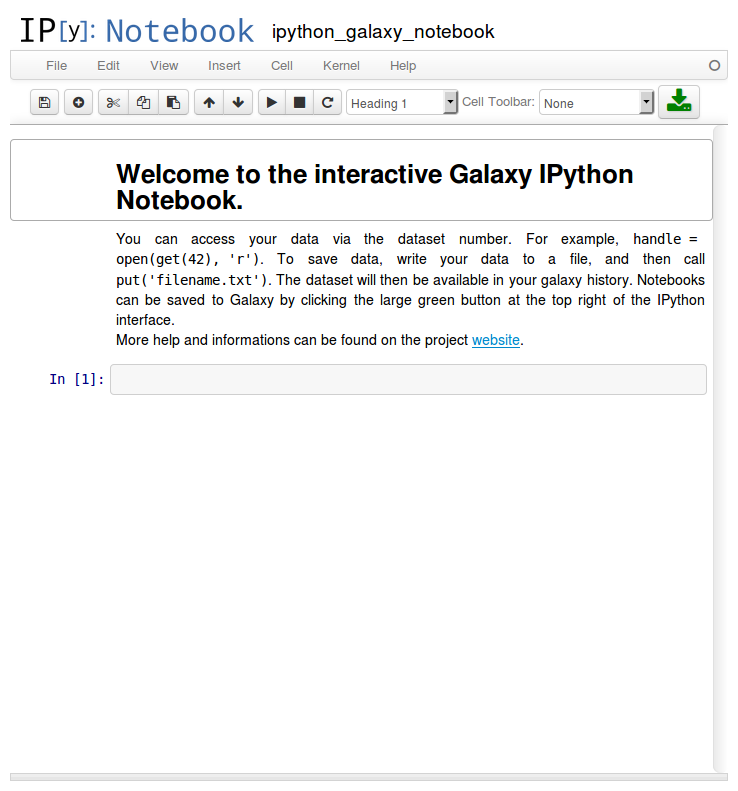
\includegraphics[width=\textwidth]{./ipy-nogx.png}
\end{frame}
\begin{frame}{... Inside of Galaxy}
	% TODO: New screenshot with Numpy/Scipy/
    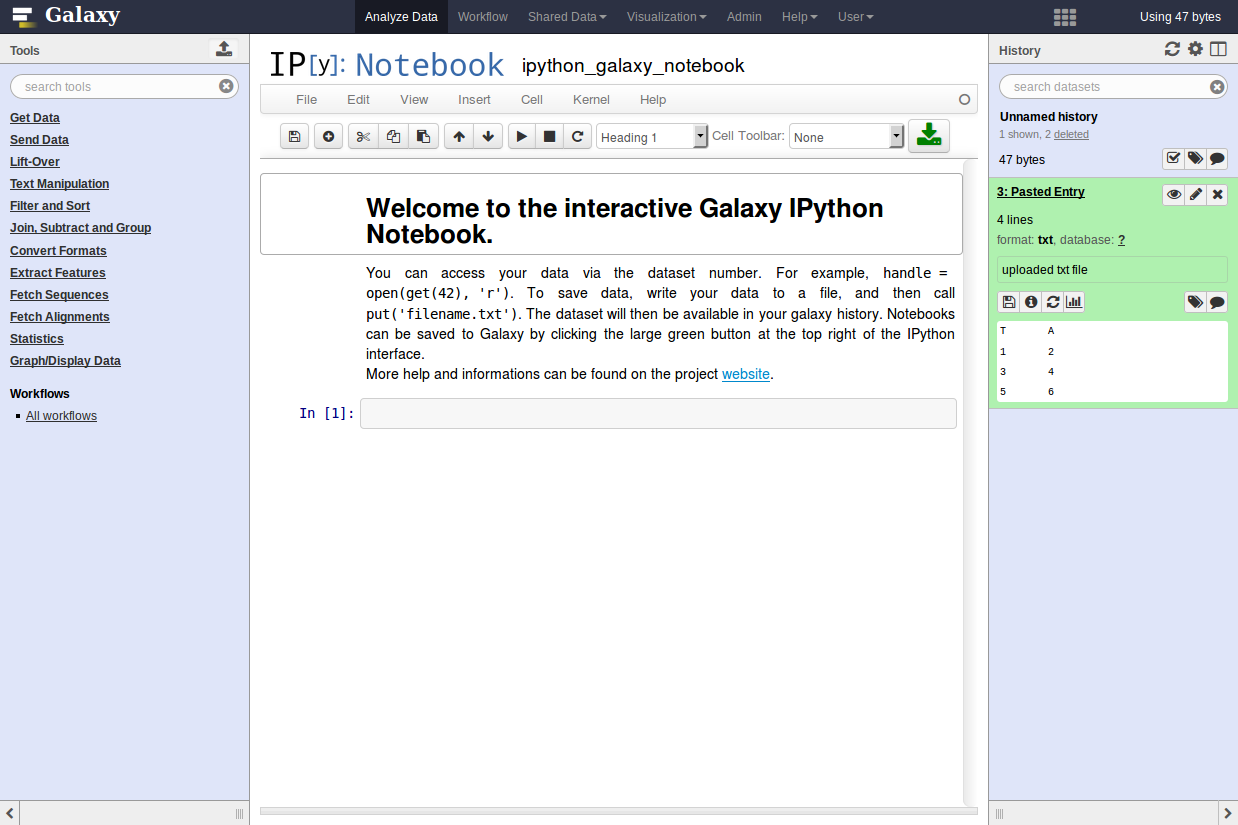
\includegraphics[width=\textwidth]{./ipy-gx.png}
\end{frame}


\section{Demo}
\begin{frame}{IE Demonstration}
	%live demonstration or picture for picture?
    % TODO: Screencast as well
	\begin{itemize}
    	\item We'll demonstrate some analysis ...
        \item \url{www.youtube.com/watch?v=UOFFkDuJxgk}
    \end{itemize}
\end{frame}

\section{How?}
  \begin{frame}{How does this magic work?}
      \centering
	  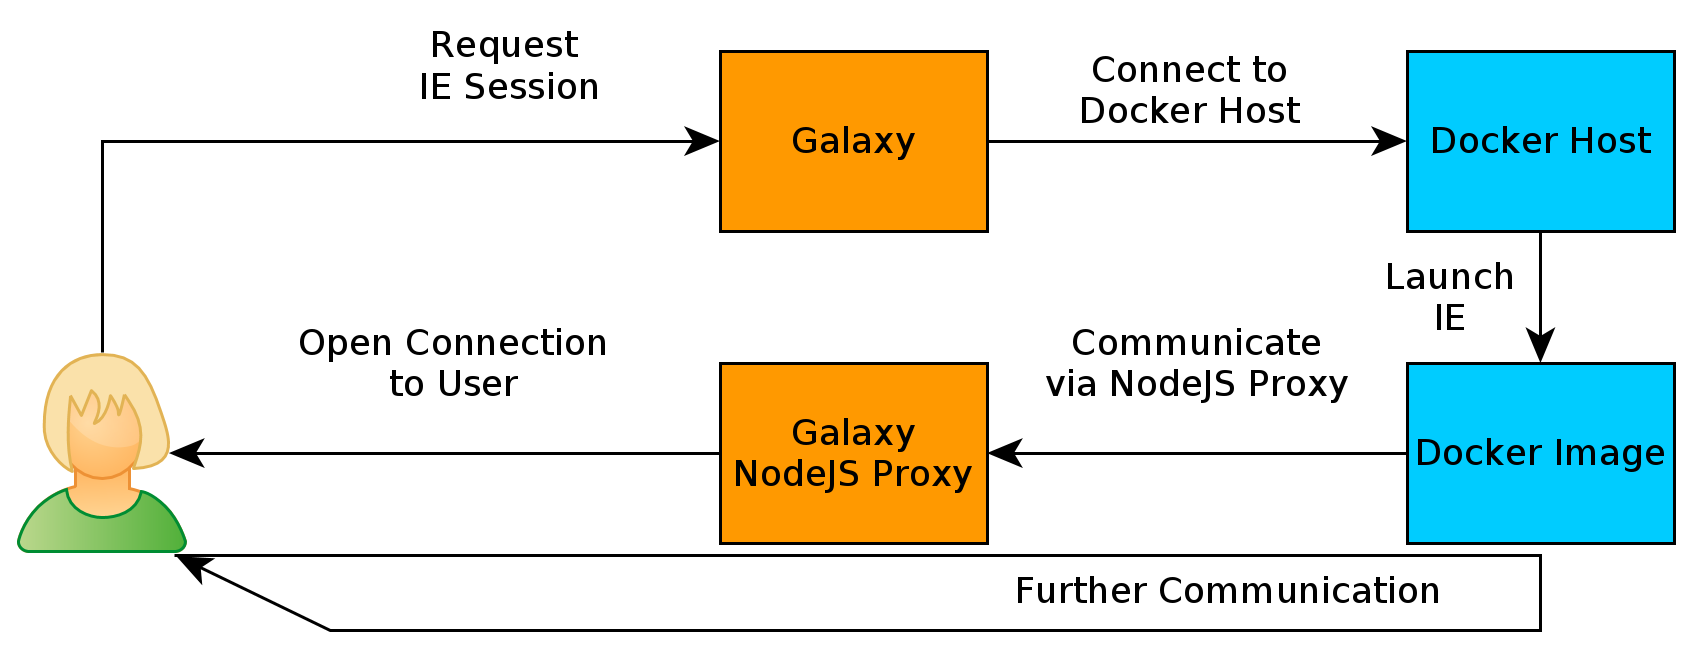
\includegraphics[width=\textwidth,height=0.8\textheight,keepaspectratio]{gx-ie.png}
  \end{frame}


\section{Who?}
  \begin{frame}{Who should use IEs?}
      \begin{itemize}
          \item Everyone!
          \item IPython/RStudio are great for bioinformaticians and Data Scientists 
          \item The upcoming iobio visualization IEs are great for Life Scientists 
      \end{itemize}
  \end{frame}

\section{Why?}
  \begin{frame}{Why use IEs instead of ... Galaxy Tools/Viz?}
      \begin{itemize}
          \item Tools are not one-size-fits-all
          \item Visualisations are restrictive
          \item Complete freedom!
      \end{itemize}
  \end{frame}
  
  \begin{frame}{Why use IEs instead of ... ``normal'' service deployments?}
      \begin{itemize}
          \item IPython Notebooks are stored as history elements
          \item Notebooks are re-runnable, maintaining reproducibility
          %\item Closer to Galaxy -- faster data analysis
          \item API interactions required to access data are all 100\% transparent
          \item Transparently integrates with standard Galaxy deployments and authentication schemes
          \item Notebooks are rendered into HTML for easy viewing/sharing, without launching an IE
      \end{itemize}
  \end{frame}
  
\section{Use Cases}
  \subsection{Teaching}
  \begin{frame}{Teaching}
    \begin{itemize}
      \item Ideal for teaching:
      	\begin{itemize}
          \item Researchers
          \item Bioinformatics
          \item Data Wrangling
          \item and Scientific Programming
        \end{itemize}
      \item Share notebooks with students inside of Galaxy
      \item Use ``literate programming'' in IPython to teach students how analyses work, line-by-line
    \end{itemize}
  \end{frame}
  
  \subsection{Research}
  \begin{frame}{Research}
    \begin{itemize}
      \item Reproducible and transparent scripts
      \item Share ``hotfix'' scripts  easily between bioinformaticians and researchers
    \end{itemize}
  \end{frame}

  \begin{frame}{Development}
    \begin{itemize}
      \item	Rapidly prototype new scripts and tools for your organisation
      \item Immediately test them on your large, real datasets 
      \item Does an existing visualisation not meet your goals? Build a new one immediately in IPython/RStudio.
    \end{itemize}
  \end{frame}
  
\section{Available IEs}
\begin{frame}{IEs}
  Available Now
  \begin{itemize}
    \item IPython (included in Galaxy 15.05/Cloudman)
    \item RStudio (coming in Galaxy 15.07)
  \end{itemize}

  Coming Soon
  \begin{itemize}
    \item iobio BAM
    \item iobio VCF
  \end{itemize}
  
  In the Works
  \begin{itemize}
    \item Apache Zeppelin
    \item WebApollo
    \item Jupyter 3/4 (Python/R/Julia/Perl/Ruby)
  \end{itemize}
\end{frame}

\subsection{IPython}
\begin{frame}{IPython IE Features}
  \begin{itemize}
  	\item Baked in Bioblend access to Galaxy
  	\item Easily get data from/put data into Galaxy
    \item Bash and R ``magics''
    \item Pre-installed: numpy biopython scikit-learn pandas scipy sklearn-pandas bioblend matplotlib patsy pysam khmer dendropy ggplot mpld3 sympy rpy2
  \end{itemize}
\end{frame}

\subsection{RStudio}
\begin{frame}{RStudio IE Features}
  \begin{itemize}
  	\item Easily get data from/put data into Galaxy
    \item R version 3.2.1
    \item Knitr/Sweave available
    \item R Packages: RCurl, XML, markdown, shiny, ggvis, dplyr, ggplot2, plyr, reshape2, devtools, RODBC, maps, pheatmap, readr, tidyr, dplyr, RJSONIO, shinyapps, knitr
    \item Bioconductor: edgeR, Rgraphviz, biomaRt, topGO, limma, DESeq2, cummeRbund, Biostrings, GenomicRanges, Rsamtools, affy
  \end{itemize}
\end{frame}

\section{Thanks}
\begin{frame}{Thanks}
A big thank you to:
 \begin{itemize}
   \item John Chilton for his help getting the IE codebase merged into Galaxy originally
   \item Enis Afgan for getting the IEs into Cloudman
   \item the Galaxy Team for supporting this exciting new feature we've developed.
  \end{itemize}
\end{frame}

\section{Q\&A}
\begin{frame}{Q\&A}

\begin{figure}
\centering
\begin{minipage}{.5\textwidth}
  \centering
  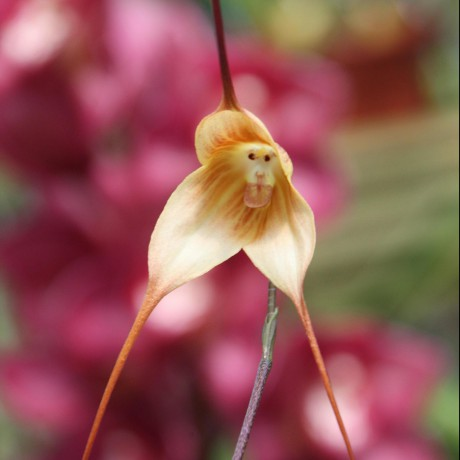
\includegraphics[width=.8\textwidth]{bgruening.png}\\
  \texttt{github.com/bgruening}
\end{minipage}%
\begin{minipage}{.5\textwidth}
  \centering
  
\includegraphics[width=.8\textwidth]{erasche.png}\\
  \texttt{github.com/erasche}
\end{minipage}
\begin{itemize}
	\item IPython \url{http://bit.ly/gxIEipython}
    \item RStudio \url{http://bit.ly/gxIErstudio}
\end{itemize}

\end{figure}


\end{frame}

\end{document}